% !TEX TS-program = pdflatex
% !TEX encoding = UTF-8 Unicode

% Matthew Urffer Master Thesis
% 

%%%%%%%%%%%%%%%%%%%%%%%%%%%%%%%%%%%%%%%%%%%%%%%%%%%%%%%%%%%%%%%%%%%%%%%%%%%%%%%
%                                                                             %
%					                         PREAMBLE                                   %
%                                                                             %
%%%%%%%%%%%%%%%%%%%%%%%%%%%%%%%%%%%%%%%%%%%%%%%%%%%%%%%%%%%%%%%%%%%%%%%%%%%%%%%
\documentclass[compress]{beamer}

\mode<presentation>
{
  %\usetheme{Boadilla}
  \usetheme{Frankfurt}
  \usecolortheme{crane}
  \setbeamercovered{transparent}
}

% Package Setup
%%%%%%%%%%%%%%%%%%%%%%%%%%%%%%%%%%%%%%%%%%%%%%%%%%%%%%%%%%%%%%%%%%%%%%%%%%
%                                                                        %
%                                 PREAMBLE                               %
%                                                                        %
%%%%%%%%%%%%%%%%%%%%%%%%%%%%%%%%%%%%%%%%%%%%%%%%%%%%%%%%%%%%%%%%%%%%%%%%%%

%% PACKAGES
\usepackage[]{lineno}
\usepackage{fancyvrb}
\usepackage{appendixnumberbeamer}
\usepackage{amsmath}
\usepackage{microtype}
\usepackage{algorithmic}

%% GRAPHICS RELATED
\usepackage{xcolor}
\usepackage{graphicx}
\usepackage[outdir=./tmp/]{epstopdf}
\graphicspath{{./figures/}{./tmp/}}
\DeclareGraphicsExtensions{.eps, .pdf, .jpeg, .png}

%% CAPTION SETUP
\usepackage{float}
\usepackage[font=footnotesize]{caption}
\usepackage[font=small]{subcaption}
\captionsetup{belowskip=12pt,aboveskip=4pt}

%% TABLES
\usepackage{multicol}
\usepackage{multirow}
\usepackage{array}				% Table Stuff
\usepackage{arydshln}
\usepackage{rotating}
\newcolumntype{C}[1]{>{\centering}m{#1}}
%% BIBLIOGRAPHY
\bibliographystyle{ieeetr}

%% UNITS
\usepackage{siunitx}

%% EQUATIONS
%\numberwithin{equation}{section}

%%%%%%%%%%%%%%%%%%%%%%%%%%%%%%%%%%%%%%%%%%%%%%%%%%%%%%%%%%%%%%%%%%%%%%%%%%%
%                                                                         %
%                             Listing Setup                               %
%                                                                         %
%%%%%%%%%%%%%%%%%%%%%%%%%%%%%%%%%%%%%%%%%%%%%%%%%%%%%%%%%%%%%%%%%%%%%%%%%%%
\usepackage{listings}
\lstset{ %
    language=C++,
    basicstyle=\footnotesize\ttfamily,
    numbers=left,
    numberstyle=\tiny\color{gray},
    stepnumber=2,
    numbersep=5pt,
    backgroundcolor=\color{white},
    showspaces=false,
    showstringspaces=false,
    showtabs=false,
    frame=single,
    rulecolor=\color{black},
    tabsize=2,
    breaklines=true,
    breakatwhitespace=false,
    title=\lstname,
    keywordstyle=\color{blue},
    commentstyle=\color{green},
    stringstyle=\color{orange}
}
\DeclareCaptionFont{white}{\color{white}}
\DeclareCaptionFormat{listing}{\colorbox[cmyk]{0.43, 0.35, 0.35, 0.01}{\parbox{\dimexpr\textwidth-2\fboxsep\relax}{#1#2#3}}}
\captionsetup[lstlisting]{format=listing,labelfont=white,textfont=white,singlelinecheck=false,margin=0pt,font={bf,footnotesize}}
%\lstnewenvironment{code}[1][]%
%{ \noindent\minipage{\linewidth}
%	\lstset{#1}
%}
%{\endminipage}
%% USER COMMANDS
\usepackage{isotope}
\newcommand{\iso}{\isotope}
\newcommand{\figurewidth}{\textwidth}
\newcommand{\micron}{$\mu$m}



% Preamble / Frst Size
%\setbeamersize{text margin left=5mm, text margin right 5mm}
\title[Matthew Urffer Master's Thesis] {Design of a Neutron Detector Capable of Replacing ${}^3$He Detectors Utilizing Thin Polymeric Films}
\subtitle{Master's Thesis Defense}
\author[] {Matthew Urffer\inst{1} }
\institute[University of Tennessee] { 
  \inst{1}%
  Department of Nuclear Engineering\\
  University of Tennessee, Knoxville, TN
}

\date[] {November 8th, 2012}
\pgfdeclareimage[height=0.5cm]{university-logo}{../images/utwordmarkhorz.png}
\logo{\pgfuseimage{university-logo}}


% Delete this, if you do not want the table of contents to pop up at
% the beginning of each subsection:
\AtBeginSection[]
{
  \begin{frame}<beamer>{}
    \frametitle{\insertsectionhead}
    \begin{multicols}{2}
  % \tableofcontents[currentsubsection,hideothersubsections,sectionstyle=show/hide,subsectionstyle=show/shaded,]
    \tableofcontents[currentsection] 
    \end{multicols}
  \end{frame}
}


% If you wish to uncover everything in a step-wise fashion, uncomment
% the following command: 
%\beamerdefaultoverlayspecification{<+->}


\begin{document}

\begin{frame}
  \titlepage
\end{frame}

\begin{frame}{Table of Contents}
  \begin{multicols}{2}
    %\tableofcontents[currentsection,pausesections]
    \tableofcontents[currentsection]
    \end{multicols}
\end{frame}


%%%%%%%%%%%%%%%%%%%%%%%%%%%%%%%%%%%%%%%%%%%%%%%%%%%%%%%%%%%%%%%%%%%%%%%%%%%%%%%
%                                                                             %
%                             START OF CONTENT                                %
%                                                                             %
%%%%%%%%%%%%%%%%%%%%%%%%%%%%%%%%%%%%%%%%%%%%%%%%%%%%%%%%%%%%%%%%%%%%%%%%%%%%%%%
\subsection{Radiation Portal Monitors}
%%%%%%%%%%%%%%%%%%%%%%%%%%%%%%%%%%%%%%%%%%%%%%%%%%%%%%%%%%%%%%%%%%%%%%%%%%%%%%%
\begin{frame}{U.S. Border Traffic}
\begin{columns}[onlytextwidth]
\begin{column}{0.45\textwidth}
  \begin{itemize}
  \item Every day 932,456 people cross into the U.S. \cite{cpb_typical_2012}
    \begin{itemize}
    	\item 259,191 by air
	\item 48,073 by sea
	\item 621,874 by land
    \end{itemize}
  \item 64,483 truck, rail and sea containers \cite{cpb_typical_2012}
 \item 253,821 privately-owned vehicles \cite{cpb_typical_2012}
  \end{itemize}
\end{column}
\begin{column}{0.45\textwidth}
  \begin{figure}[ht]
    \vspace*{-3cm}
		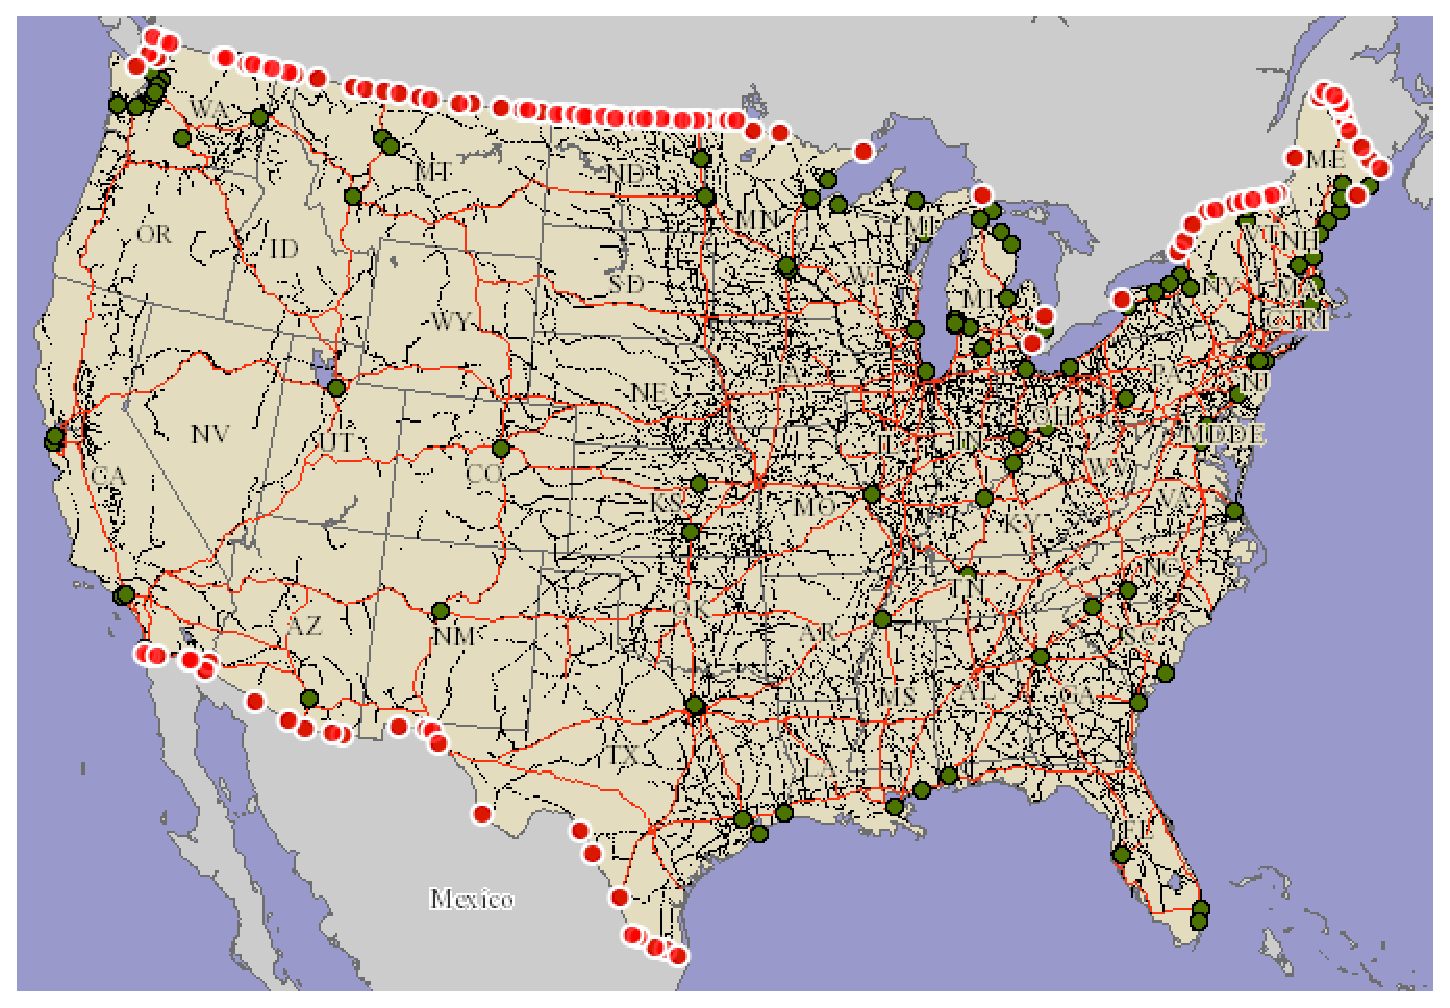
\includegraphics[width=\textwidth]{PortalEntryMap.eps}
  \end{figure}
\end{column}
\end{columns}
\end{frame}

%%%%%%%%%%%%%%%%%%%%%%%%%%%%%%%%%%%%%%%%%%%%%%%%%%%%%%%%%%%%%%%%%%%%%%%%%%%%%%%
\begin{frame}{Radiation Portal Monitors}
\begin{columns}[onlytextwidth]
	\begin{column}{0.45\textwidth}
  	\begin{itemize}
  		\item Radiation portal monitors (RPMs) are passive radiation detectors
  		\item {
  			 RPMs are currently   ${}^3$He based detectors
  			\center
    		${}^3He +n \to p +{}^3H$
    	}
  		\item Shortage of ${}^3$He, so alternatives are being explored
		  \item ${}^6Li + n \to {}^3H + \alpha$    
  		\end{itemize}
	\end{column}
	\begin{column}{0.5\textwidth}
		\begin{figure}
    \vspace*{-3cm}
      \centering
			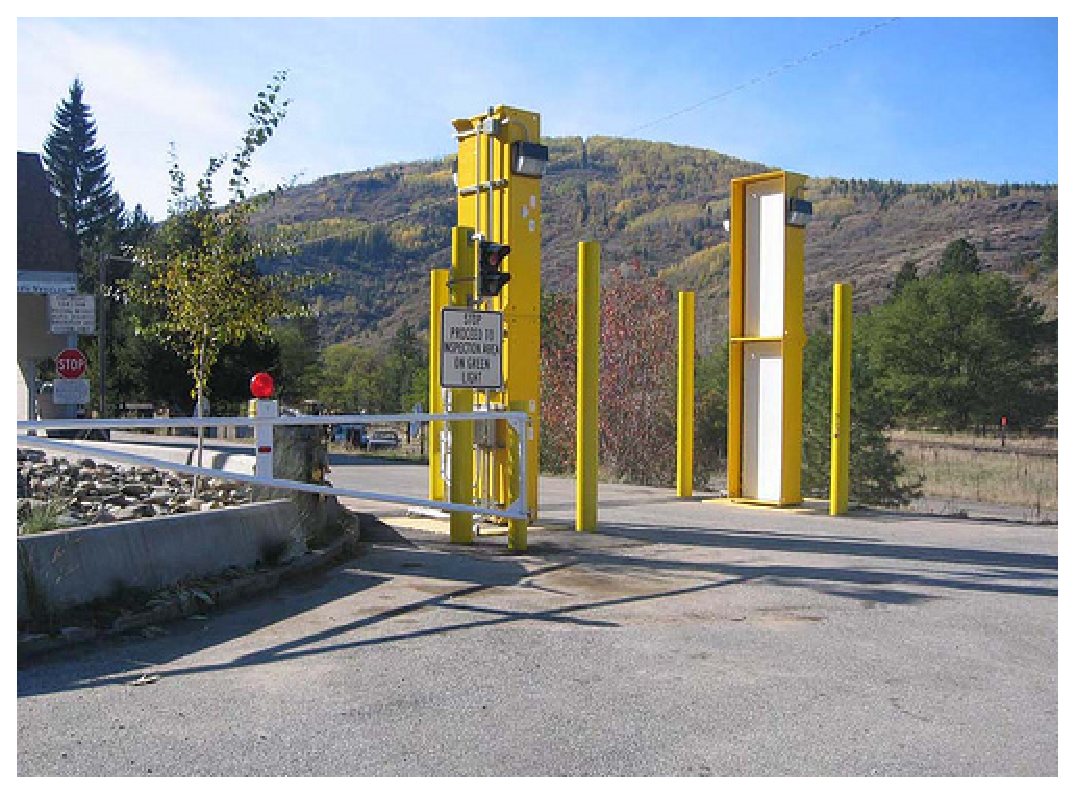
\includegraphics[width=\textwidth]{RPM8_Installed.eps}
    \end{figure}
	\end{column}
\end{columns}
\end{frame}
%%%%%%%%%%%%%%%%%%%%%%%%%%%%%%%%%%%%%%%%%%%%%%%%%%%%%%%%%%%%%%%%%%%%%%%%%%%%%%%

\subsection{Detector Requirements}
%%%%%%%%%%%%%%%%%%%%%%%%%%%%%%%%%%%%%%%%%%%%%%%%%%%%%%%%%%%%%%%%%%%%%%%%%%%%%%%
\begin{frame}{Detector Requirements}
DHS / DNDO (along with PNNL) has determined a set of objectives that replacement technologies should meet:
\begin{table}
	\small
	\begin{tabular}{ m{5cm} m{5cm} }
	Parameter & Specification \\
	\hline
	\hline
	Absolute neutron detection efficiency & 2.5 cps/ng of ${}^{252}Cf$ (in specified test configuration) \\
	Intrinsic gamma-neutron detection efficiency & $ \epsilon_{int,\gamma n}\leq 10^{-6}$ \\
	Gamma absolute rejection ratio for neutrons (GARRn) & $ 0.9 \leq \text{ GARRn }\leq$ 1.1 at 10 mR/h exposure \\
	Cost &  \$ 30,000 per system \\
	\hline
	\end{tabular}
\end{table}
\hyperlink{PNNLCriteria}{\beamerbutton{Detailed Criteria}}
\label{DHSCriteria}
\end{frame}

%%%%%%%%%%%%%%%%%%%%%%%%%%%%%%%%%%%%%%%%%%%%%%%%%%%%%%%%%%%%%%%%%%%%%%%%%%%%%%%
%                                                                             %
%                                PREVIOUS WORK                                %
%                                                                             %
%%%%%%%%%%%%%%%%%%%%%%%%%%%%%%%%%%%%%%%%%%%%%%%%%%%%%%%%%%%%%%%%%%%%%%%%%%%%%%%
\subsection{Previous Work}

%%%%%%%%%%%%%%%%%%%%%%%%%%%%%%%%%%%%%%%%%%%%%%%%%%%%%%%%%%%%%%%%%%%%%%%%%%%%%%%
\begin{frame}[fragile]{Replacement Technologies}
\begin{columns}[onlytextwidth]
\begin{column}{0.55\textwidth}
\begin{itemize}
	\small
	\item Boron Straw Tubes (Proportional Technology) \cite{kouzes_boron-lined_2012}
	\begin{itemize}
    %\tiny
		\item Count rate meets requirements
		\item Gamma rejection is estimated to be $4x10^{-9}$
		\item GARRn within desired range
	\end{itemize}
	\small
	\item LiF:ZnS coated Paddles (IAT) \cite{kouzes_lithium_2010}
	\begin{itemize}
    %\tiny
		\item Did not fulfill the neutron count rate
		\item Adequate gamma ray rejection
		\item Passed the GARRn
	\end{itemize}
\end{itemize}
\end{column}
\begin{column}{0.4\textwidth}
	\begin{figure}
    \centering
    \begin{subfigure}[b]{\textwidth}
      \centering
		  \includegraphics[height=0.25\textheight]{B10StrawFibers.eps}
      \caption{ ${}^{10}$B Straw Fibers}
      \label{fig:B10StrawFibers}
    \end{subfigure}

    \begin{subfigure}[b]{\textwidth}
      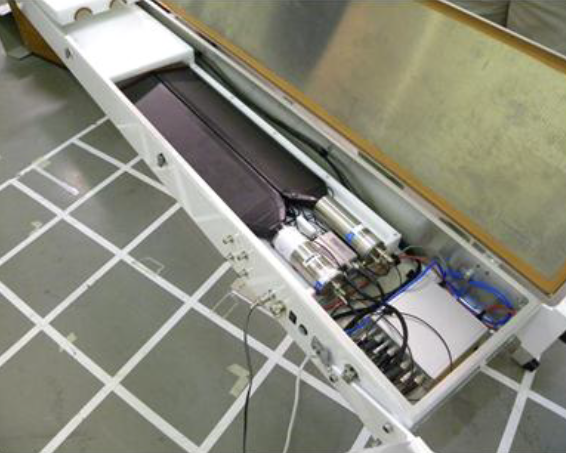
\includegraphics[height=0.25\textheight]{IATImage}
      \caption{${}^6$LiF:ZnS Paddle}
      \label{fig:LifZnSPaddle}
    \end{subfigure}
	\end{figure}
\end{column}
\end{columns}
\end{frame}

% !TEX TS-program = pdflatex
% !TEX encoding = UTF-8 Unicode

% Matthew Urffer Master Thesis
% 
% Methods
%
\section{Spectra Methods}

%%%%%%%%%%%%%%%%%%%%%%%%%%%%%%%%%%%%%%%%%%%%%%%%%%%%%%%%%%%%%%%%%%%%%%%%%%%%%%%
%                                                                             %
%                                   FACILITIES                                %
%                                                                             %
%%%%%%%%%%%%%%%%%%%%%%%%%%%%%%%%%%%%%%%%%%%%%%%%%%%%%%%%%%%%%%%%%%%%%%%%%%%%%%%

\subsection{Facilities}
%%%%%%%%%%%%%%%%%%%%%%%%%%%%%%%%%%%%%%%%%%%%%%%%%%%%%%%%%%%%%%%%%%%%%%%%%%%%%%%
\begin{frame}{Button Sources}
	\centering
	Alpha Sources
	\begin{table}[h]
		\tiny
		\begin{tabular}{c | c c}
		Source & Half-Life & Energy (MeV) \\
		\hline
		\hline
		${}^{232}$Th & $1.4\times10^{10}$ yr & 4.012 \\
		${}^{240}$Pu & $6.5\times10^{3}$ yr & 5.17 (76\%) 5.12 (24\%) \\
		${}^{241}$Am & 433 yr & 5.48 (85\%) 5.44 (12\%) \\
		${}^{239}$Pu, ${}^{241}$Am, ${}^{244}$Cm  & various & various \\
		\end{tabular}
	\end{table}
	Beta Sources
	\begin{table}[h]
		\tiny
		\begin{tabular}{c | c c}
		Source & Half-Life & Endpoint Energy (MeV)\\
		\hline
		\hline
		${}^{14}$C &  5,730 yr & 0.156 \\
		${}^{36}$Cl & $3.08\times10^{5}$ yr & 0.714 \\
		${}^{36}$Ni &  92 yr & 0.067 \\
		${}^{99}$Tc & $2.12\times10^{5}$ yr & 0.292 \\
		\end{tabular}
	\end{table}
\end{frame}

%%%%%%%%%%%%%%%%%%%%%%%%%%%%%%%%%%%%%%%%%%%%%%%%%%%%%%%%%%%%%%%%%%%%%%%%%%%%%%%
\begin{frame}{Gamma Irridiator}
\begin{columns}[onlytextwidth]
\begin{column}{0.45\textwidth}
	\begin{itemize}
		\item Desire a 10 mR/hr Gamma Field
		\item Solution is a 100 $\mu$Ci ${}^{60}$Co source
		\item Shielded by lead
	\end{itemize}
\end{column}
\begin{column}{0.45\textwidth}
	\centering
	\begin{figure}
		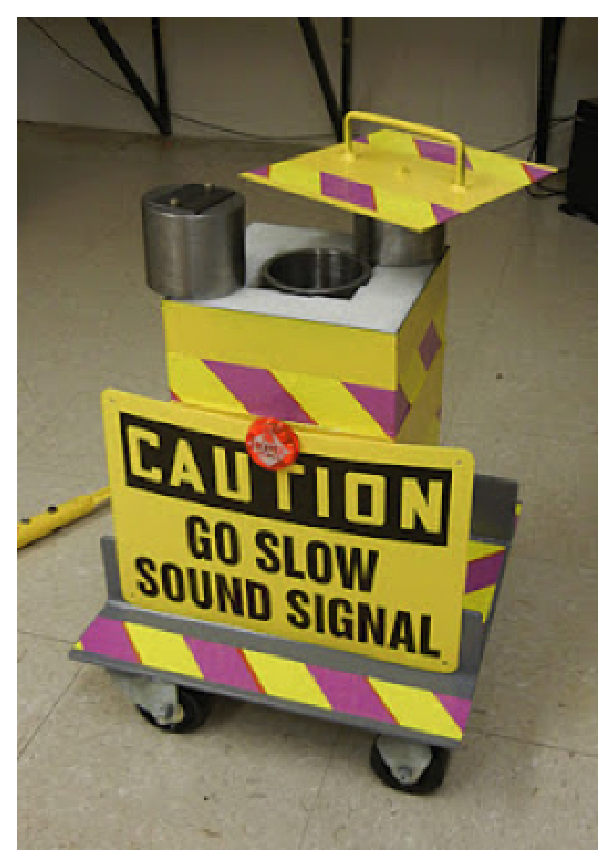
\includegraphics[width=0.8\textwidth]{GammaIrridiator.eps}
		\label{fig:GammaIrridiator}
		\caption{Gamma Irridiator}
	\end{figure}
\end{column}
\end{columns}
\end{frame}

%%%%%%%%%%%%%%%%%%%%%%%%%%%%%%%%%%%%%%%%%%%%%%%%%%%%%%%%%%%%%%%%%%%%%%%%%%%%%%%
\begin{frame}{Neutron Irridiator}
\begin{columns}[onlytextwidth]
\begin{column}{0.45\textwidth}
	\small
	\begin{itemize}
		\item Source is 0.59 $\mu$g ${}^{252}$Cf
		\item Encased in HDPE Box
		\item Two detector wells
		\begin{itemize}
			\tiny
			\item Lead Well
			\item Cadmium Well
		\end{itemize}
	\end{itemize}
\end{column}
\begin{column}{0.45\textwidth}
	\begin{figure}
		\centering
		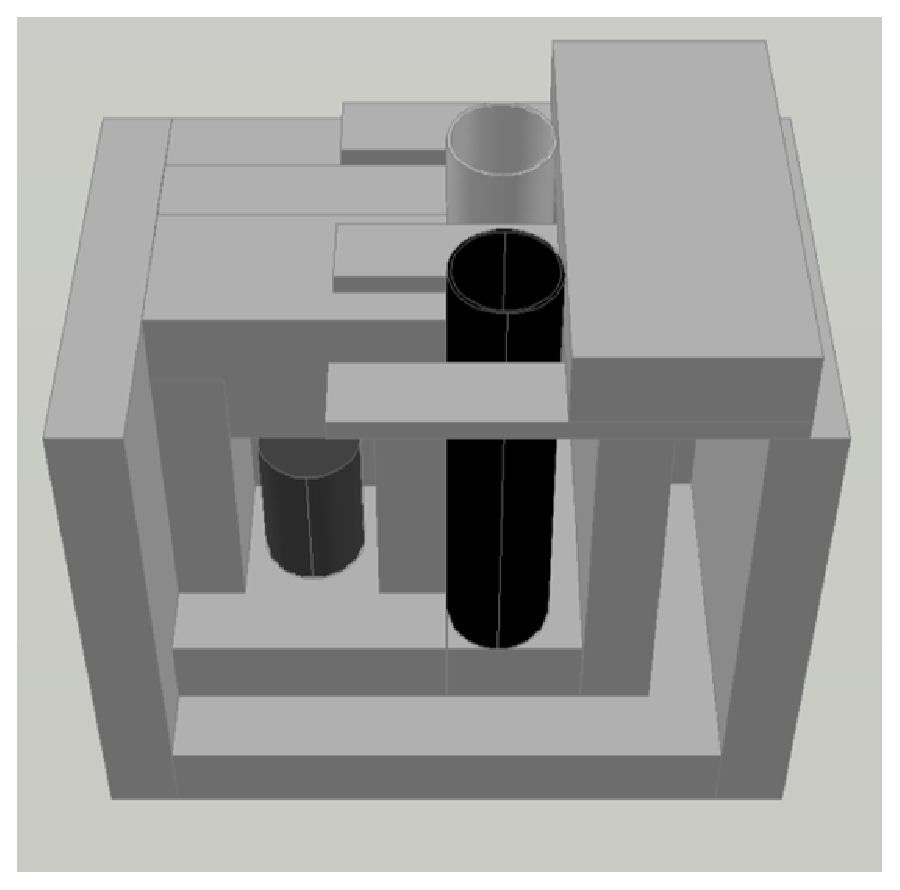
\includegraphics[height=0.25\textheight]{NeutronIrridiator_CAD.eps}
		\caption{CAD Rendering of Neutron Irridiator}
		\label{fig:NeutronIrridiatorCAD}
		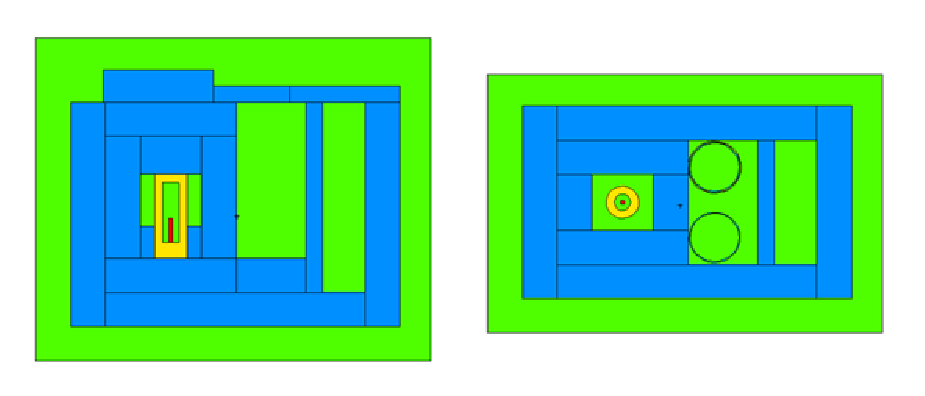
\includegraphics[height=0.25\textheight]{NeutronIrridiator_MCNP.eps}
		\caption{MCNPX Rendering of Neutron Irridiator}
		\label{fig:NeutronIrridiatorMNCPX}
	\end{figure}
\end{column}
\end{columns}
\end{frame}

%%%%%%%%%%%%%%%%%%%%%%%%%%%%%%%%%%%%%%%%%%%%%%%%%%%%%%%%%%%%%%%%%%%%%%%%%%%%%%%
\begin{frame}{Neutron Irridiator (Spectra)}
\begin{columns}[onlytextwidth]
\begin{column}{0.45\textwidth}
	\begin{itemize}
		\small
		\item Lead Well
		\begin{itemize}
			\tiny
			\item Neutrons of all energies
			\item Lead to match photon attenuation of cadmium
		\end{itemize}
		\small
		\item Cadmium Well
		\begin{itemize}
			\tiny
			\item Cadmium cutoff is about 0.5 eV
			\item Well response is to fast neutrons
			\item Shielding of photons from cadmium
		\end{itemize}
		\small 
		\item Subtraction is preformed between the two response to extract the response from thermal neutrons
	\end{itemize}
\end{column}
\begin{column}{0.45\textwidth}
	\begin{figure}
		\centering
		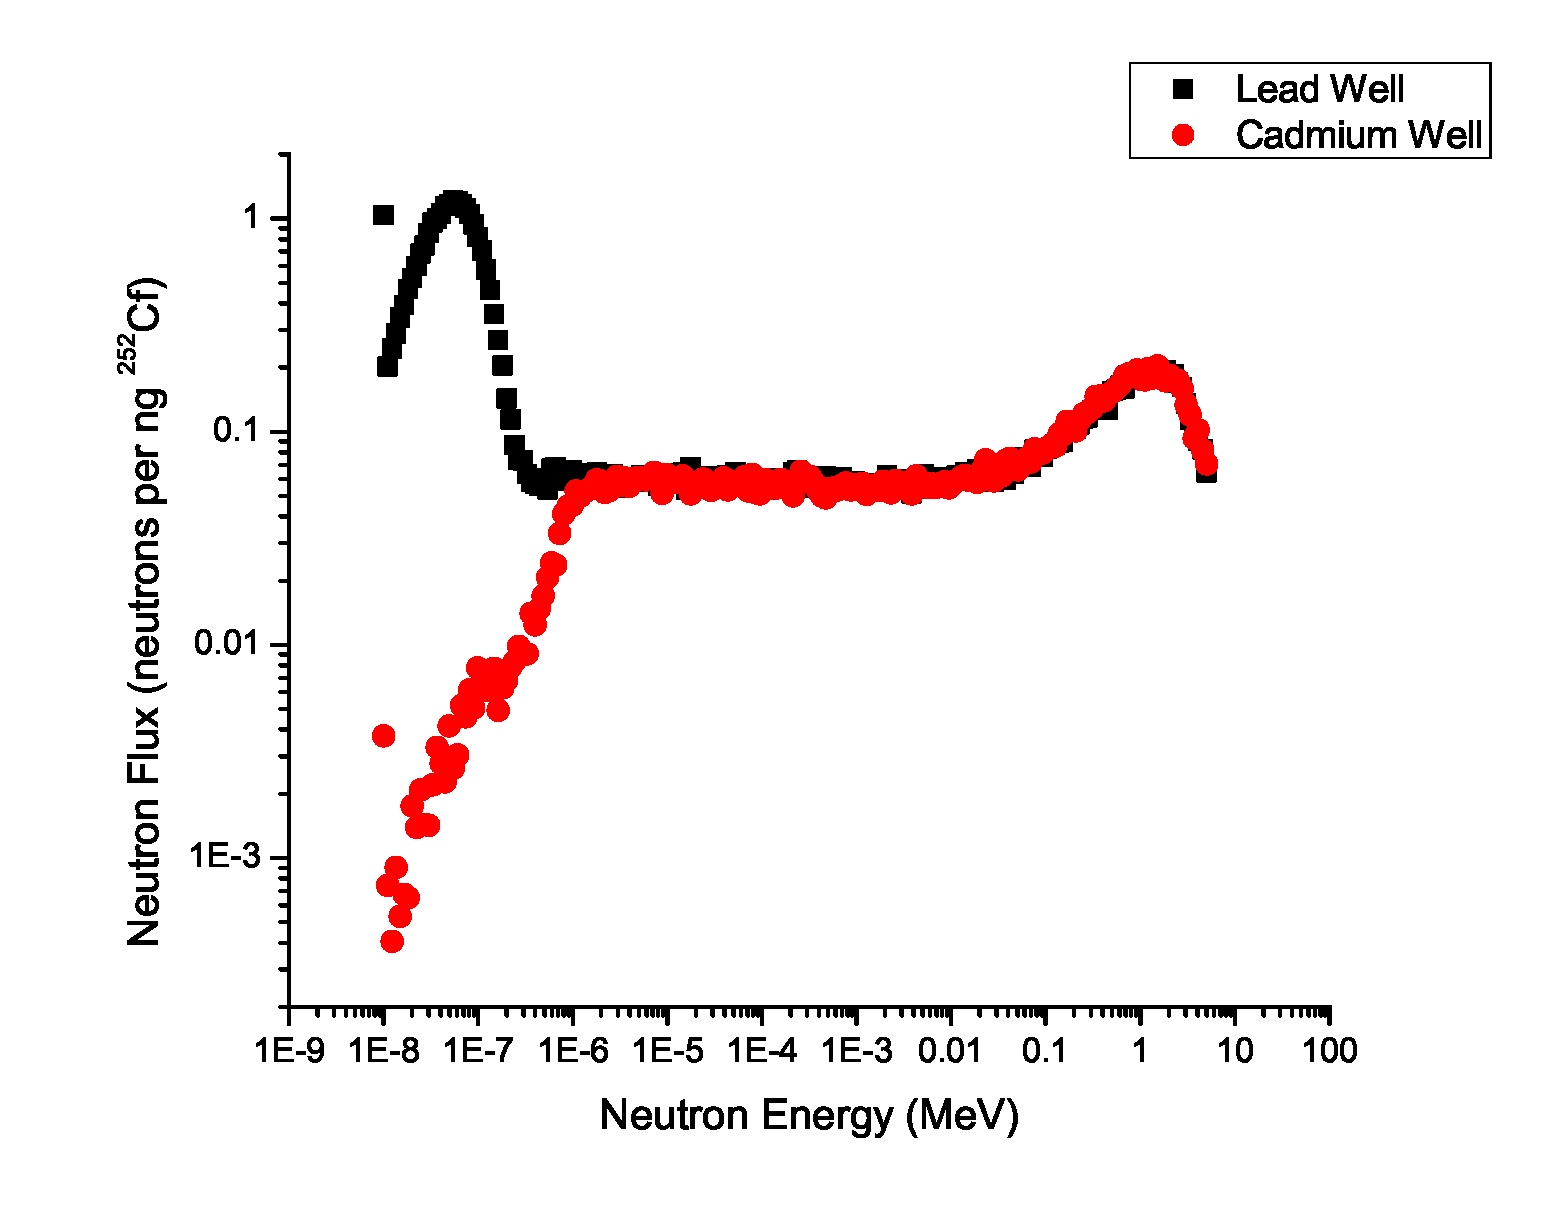
\includegraphics[width=\textwidth]{Graph19N.eps}
		\caption{Simulated Lead and Cadmium Well Spectra}
		\label{fig:SimPbCdSpectra}
	\end{figure}
\end{column}
\end{columns}
\end{frame}
%%%%%%%%%%%%%%%%%%%%%%%%%%%%%%%%%%%%%%%%%%%%%%%%%%%%%%%%%%%%%%%%%%%%%%%%%%%%%%%
\begin{frame}{Spectra Electronics}
\begin{columns}[onlytextwidth]
\begin{column}{0.45\textwidth}
	\small 
	Measurement Protocol
	\begin{itemize}
		\tiny
		\item Verify instrument gains are stable
		\begin{itemize}
			\tiny
			\item GS20 (${}^6$Li glass) is used as the standard
			\item Set voltage and coarse gain, adjust fine gain
		\end{itemize}
		\tiny
		\item Obtain a spectra from an alpha (${}^{241}$Am) 
		\item Obtain a spectra from a beta (${}^{36}$Cl)
		\item Obtain a lead well neutron spectra
		\item Obtain a cadmium well neutron spectra
		\item Obtain a gamma irridiator spectra
	\end{itemize}
\end{column}
\begin{column}{0.45\textwidth}
	\begin{figure}
		\centering
		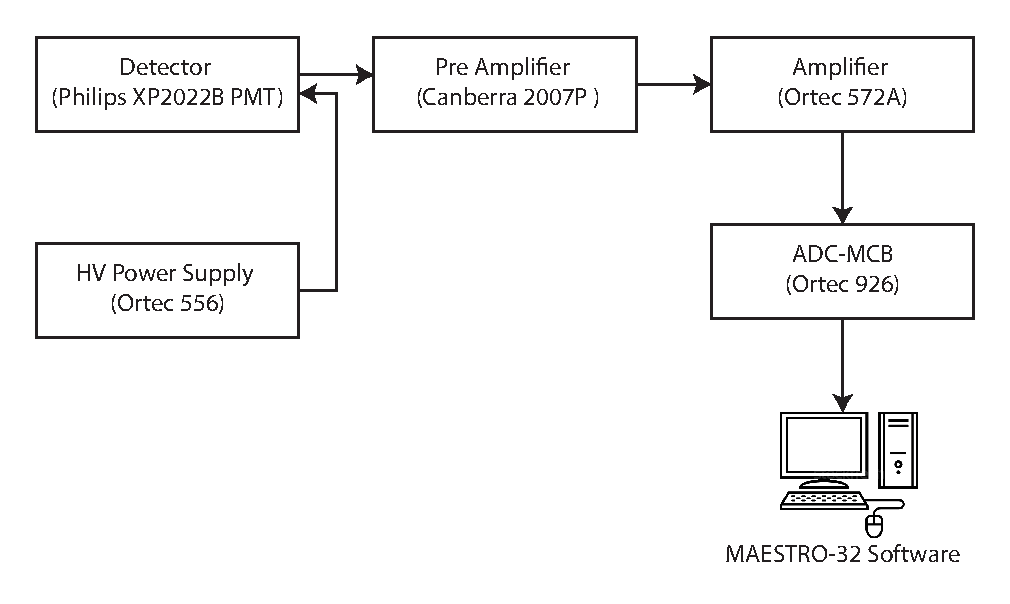
\includegraphics[height=0.5\textwidth]{ElectronicsSpectra.eps}
		\caption{Electronic Setup for Spectra}
		\label{fig:ElectronicsSpectra}
	\end{figure}
\end{column}
\end{columns}
\end{frame}
%%%%%%%%%%%%%%%%%%%%%%%%%%%%%%%%%%%%%%%%%%%%%%%%%%%%%%%%%%%%%%%%%%%%%%%%%%%%%%%
%                                                                             %
%                             ANALYSIS METHDOS                                %
%                                                                             %
%%%%%%%%%%%%%%%%%%%%%%%%%%%%%%%%%%%%%%%%%%%%%%%%%%%%%%%%%%%%%%%%%%%%%%%%%%%%%%%
\subsection{Analysis Methods}
%%%%%%%%%%%%%%%%%%%%%%%%%%%%%%%%%%%%%%%%%%%%%%%%%%%%%%%%%%%%%%%%%%%%%%%%%%%%%%%
\begin{frame}{Spectra Average}
	\begin{itemize}
		\item Thin films do not have clearly define features
		\item Spectra averages defined to create a feature
	\end{itemize}
\begin{columns}[onlytextwidth]
\begin{column}{0.45\textwidth}
	\newtheorem{thm4}{Spectra Average}
	\begin{thm4}<1->
		$$<\mu> = \frac{\int_{0}^{\infty}x\cdot f(x)dx}{\int_{0}^{\infty}f(x)dx} $$
		where:
		\begin{itemize}
			\tiny
			\item $<\mu>$ is the average of the spectra
			\item $f(x)$ is the spectra
			\item $x$ is a channel number
		\end{itemize}
	\end{thm4}
\end{column}
\begin{column}{0.45\textwidth}
	\begin{figure}
		\centering
		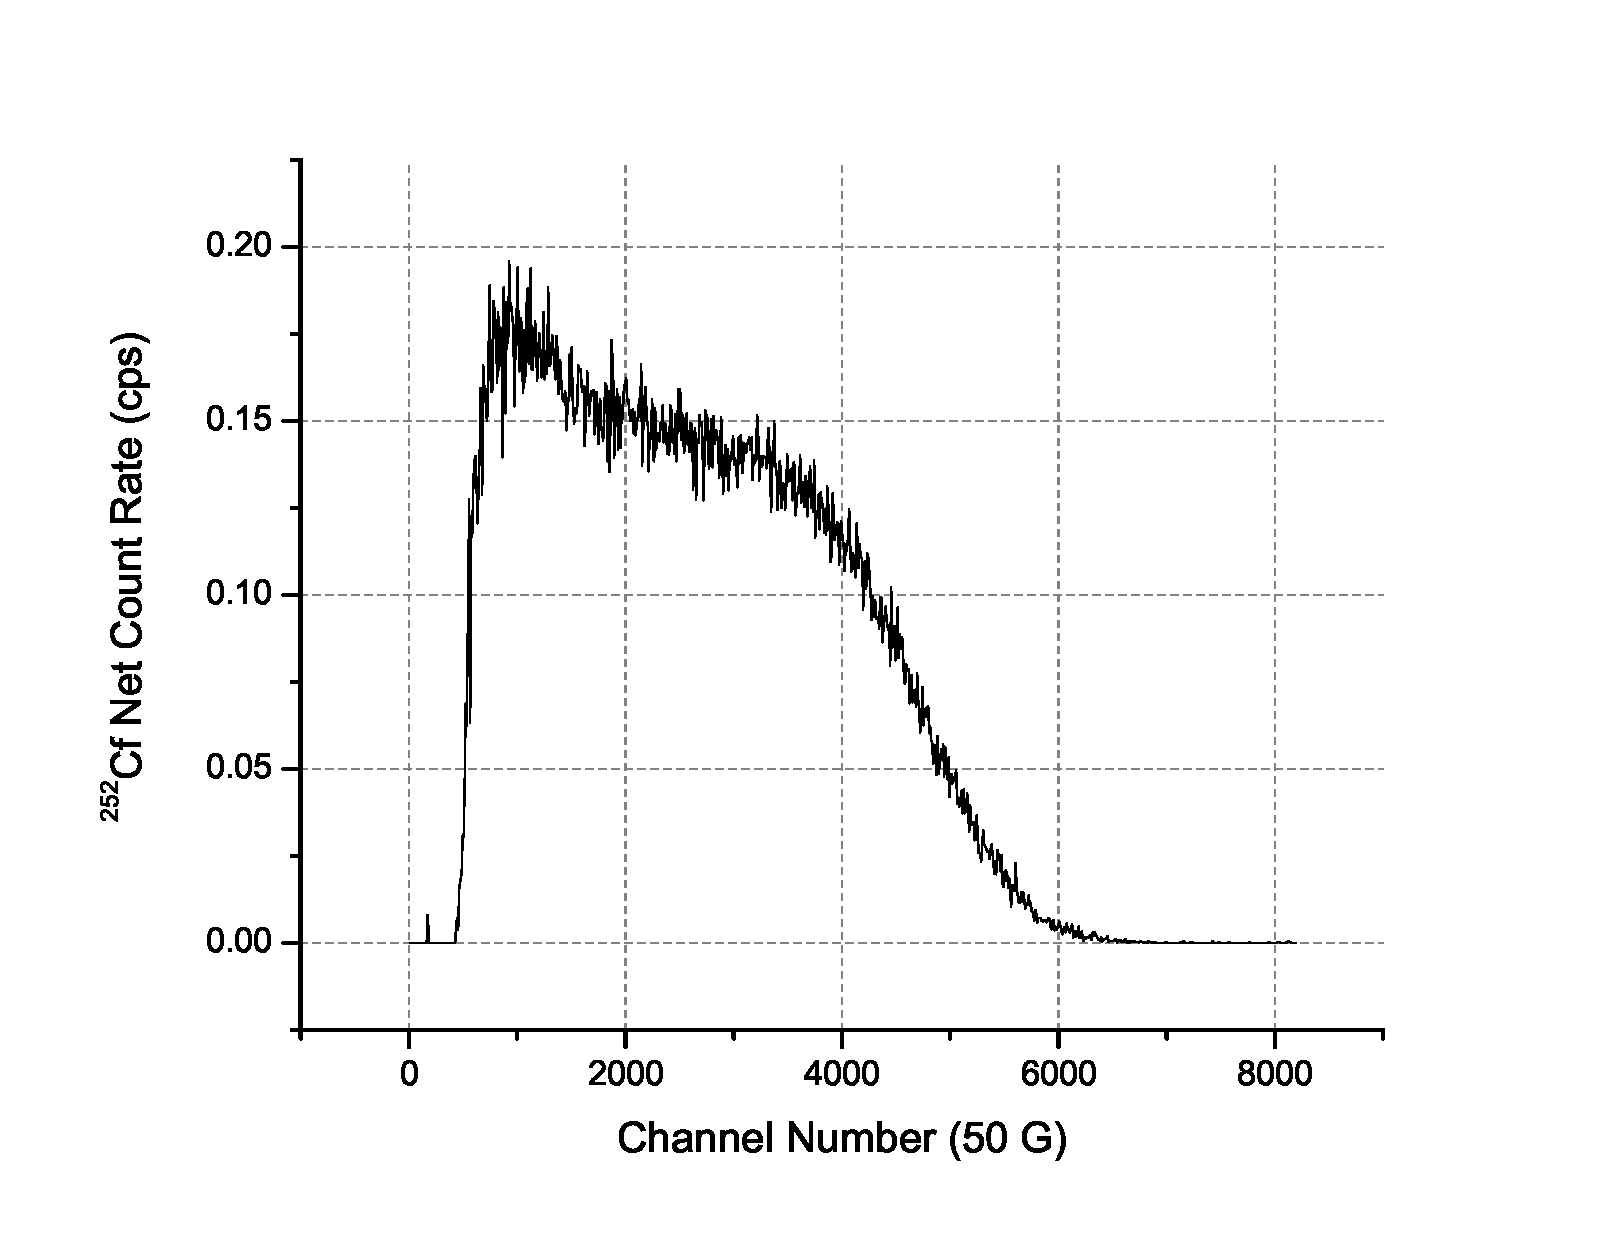
\includegraphics[width=\textwidth]{StrechedPEN-Neutron.eps}
		\caption{Example Neutron Spectra}
	\end{figure}
\end{column}
\end{columns}
\end{frame}
%%%%%%%%%%%%%%%%%%%%%%%%%%%%%%%%%%%%%%%%%%%%%%%%%%%%%%%%%%%%%%%%%%%%%%%%%%%%%%%
\begin{frame}{Pulse Height Defect}
	\newtheorem{thm5}{Pulse Height Defect}
	\begin{thm5}<1->
	\tiny
	$$ PHD_{GS20} = \frac{\dfrac{n_{peak}}{4.78\;\text{MeV}}}{\dfrac{CE_\gamma}{1.038\;\text{MeV}}} $$
		where:
		\begin{itemize}
			\tiny
			\item $PHD_{GS20}$ is the pulse height defect for GS20
			\item $n_{peak}$ is the location of the peak in the neutron spectra
			\item $CE_\gamma$ is the Compton Edge of the Gamma Spectra
		\end{itemize}
	\end{thm5}
	\newtheorem{thm6}{Pulse Height Defect (Sample)}
	\begin{thm6}<1->
	\tiny
	$$ PHD_{Sample} = PHD_{GS20} \frac{<n>_{sample}}{<n>_{GS20}} $$
		where:
		\begin{itemize}
			\tiny
			\item $PHD_{GS20}$ is the pulse height defect for GS20
			\item $<n>_{sample}$ is the average of the sample's neutron spectra
			\item $<n>_{GS20}$ is the average of GS20's neutron spectra
		\end{itemize}
	\end{thm6}
\end{frame}
%%%%%%%%%%%%%%%%%%%%%%%%%%%%%%%%%%%%%%%%%%%%%%%%%%%%%%%%%%%%%%%%%%%%%%%%%%%%%%%
\begin{frame}{Light Yield}
	\newtheorem{thm7}{Light Yield}
	\begin{thm7}<1->
	\tiny
	$$ LY_{n} = 3,800 \frac{\text{Photons}}{\text{MeV}}\frac{<n>_{sample}}{<n>_{GS20}} $$
	$$ LY_{\beta} = 3,800 \frac{\text{Photons}}{\text{MeV}}\frac{<\beta>_{sample}}{<\beta>_{GS20}} $$
	$$ LY_{\gamma} = 3,800 \frac{\text{Photons}}{\text{MeV}}\frac{<\gamma>_{sample}}{<\gamma>_{GS20}} $$
		where:
		\begin{itemize}
			\tiny
			\item $<n>_{sample}$ is the average of the sample's neutron spectra
			\item $<n>_{GS20}$ is the average of GS20's neutron spectra
			\item $<\beta>_{sample}$ is the average of the sample's beta (${}^{36}$Cl) spectra
			\item $<\beta>_{GS20}$ is the average of GS20's bet (${}^{36}$Cl) spectra
			\item $<\gamma>_{sample}$ is the average of the sample's gamma (${}^{60}$Co) spectra
			\item $<\gamma>_{GS20}$ is the average of GS20's gamma (${}^{60}$Co) spectra
		\end{itemize}
	\end{thm7}
\end{frame}
%%%%%%%%%%%%%%%%%%%%%%%%%%%%%%%%%%%%%%%%%%%%%%%%%%%%%%%%%%%%%%%%%%%%%%%%%%%%%%%
\begin{frame}
	\newtheorem{thm8}{Gamma Intrinsic Efficiency}
	\begin{thm8}<1->
		$$ \epsilon_{int,\gamma} = \frac{\int_{MLLD}^{\infty}{f(x)dx}}{\text{Particles Incident}} $$
	where:
	\begin{itemize}
		\tiny
		\item $MLLD$ is the mathematical lower level discriminator
		\item $f(x)$ is the spectra
		\item $\text{Particles Incident}$ is the number of incident particles
	\end{itemize}
	\end{thm8}
	\newtheorem{rmk1}{Mathematical Lower Level Discriminator}
	\begin{rmk1}
		\tiny
		Mathematical lower level discriminator (MLLD) is defined to be the channel at which $\epsilon_{int,\gamma} \leq 10^{-6}$
	\end{rmk1}

	\begin{itemize}
		\tiny
		\item MLLD for a film is determined from a ${}^{60}$Co measurement
		\item Source produces a 10 mR/hr field at detector surface
		\item Particles incident determined from simulation
	\end{itemize}
\end{frame}
%%%%%%%%%%%%%%%%%%%%%%%%%%%%%%%%%%%%%%%%%%%%%%%%%%%%%%%%%%%%%%%%%%%%%%%%%%%%%%%
\begin{frame}[allowframebreaks]
    \frametitle{Gamma Intrinsic Efficiency Example}
	\begin{figure}
		\centering
		\includegraphics[height=0.5\textheight]{CartoonIntEffSimple.eps}
		\caption{Determination of the MLLD for a PEN film}
		\label{fig:CartoonIntEffSimple}
	\end{figure}
%\end{frame}
%%%%%%%%%%%%%%%%%%%%%%%%%%%%%%%%%%%%%%%%%%%%%%%%%%%%%%%%%%%%%%%%%%%%%%%%%%%%%%%
%\begin{frame}{Gamma Intrinsic Efficiency Example I}
	\begin{figure}
		\centering
		\includegraphics[height=0.5\textheight]{CartoonIntEffReal.eps}
		\caption{Determination of the MLLD (Example)}
		\label{fig:ElectronicsPSD}
	\end{figure}
\end{frame}
%%%%%%%%%%%%%%%%%%%%%%%%%%%%%%%%%%%%%%%%%%%%%%%%%%%%%%%%%%%%%%%%%%%%%%%%%%%%%%%
%%%%%%%%%%%%%%%%%%%%%%%%%%%%%%%%%%%%%%%%%%%%%%%%%%%%%%%%%%%%%%%%%%%%%%%%%%%%%%%

\include{./SimMethods}
\include{./PSDMethods}
\include{./FilmPerformance}
\include{./SimPerformance}
\include{./PSDPerformance}
\section*{Conclusions}
%%%%%%%%%%%%%%%%%%%%%%%%%%%%%%%%%%%%%%%%%%%%%%%%%%%%%%%%%%%%%%%%%%%%%%%%%%%%%%%
\begin{frame}{Measurement and Data Analysis}
	\begin{itemize}
		\item A protocol has been developed for measurements
		\begin{itemize}
			\item Verification of instrument gains
			\item Neutron Measurements
			\item Gamma Measurements
			\item Various button sources
		\end{itemize}
		\item Ability to calculate MLLD necessary for $\epsilon_{int,\gamma} \le 10^{-6}$
		\item Ability to calculate light yield
	\end{itemize}
\end{frame}
%%%%%%%%%%%%%%%%%%%%%%%%%%%%%%%%%%%%%%%%%%%%%%%%%%%%%%%%%%%%%%%%%%%%%%%%%%%%%%%
\begin{frame}{Modeling}
	\begin{itemize}
		\item MCNPX modeling has been employed
		\begin{itemize}
			\item Determination of 10 mR/hr field
			\item Determination of film performance to neutrons
			\begin{itemize}
				\item Neutron Irridiator
				\item Mock up of DHS/DNDO test configuration
			\end{itemize}
		\end{itemize}
		\item Future work will be completed with GEANT4
	\end{itemize}
\end{frame}
%%%%%%%%%%%%%%%%%%%%%%%%%%%%%%%%%%%%%%%%%%%%%%%%%%%%%%%%%%%%%%%%%%%%%%%%%%%%%%%
\begin{frame}{Summary}

  \begin{itemize}
  \item
    A framework has been developed for the characterization of possible replacement technologies for radiation portal monitors
  \item
    A framework has been developed for pulse shape discrimination 
  \item
    Thin polymeric films have been demonstrated to have the necessary interaction rates for radiation portal monitors
  \end{itemize}
\begin{figure}
	\centering
		\includegraphics[width=0.3\textwidth]{Questions.eps}
\end{figure}
\end{frame}

%%%%%%%%%%%%%%%%%%%%%%%%%%%%%%%%%%%%%%%%%%%%%%%%%%%%%%%%%%%%%%%%%%%%%%%%%%%%%%%
% BILBIOLGRAPHY
\begin{frame}[plain,allowframebreaks]
\frametitle{Works Cited}
	\tiny
    \bibliography{../Zotero}
\end{frame}

% APPENDIX
\appendix
\section<presentation>*{\appendixname}
\subsection<presentation>*{Fundamental Physics}
\begin{frame}{Absorption Cross Sections}
\begin{figure}
	\centering
		\includegraphics[width=0.9\textwidth]{CrossSections.eps}
	\caption{Cross sections of selected isotopes \protect \cite{nist_neutron_2012}}
	\label{fig:CrossSections}
\end{figure}

\end{frame}




\end{document}


